\documentclass{article}

\usepackage{tikz}
\usetikzlibrary{arrows}

\begin{document}

\begin{center}
\fbox{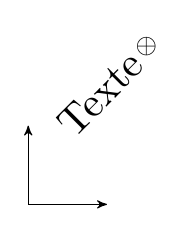
\begin{tikzpicture}
    % code de la Figure
    \draw [<->,>=stealth'] (1,0) -- (0,0) -- (0,1);
    \path (1.5,2) node{$\oplus$} node[left,scale=1.5,rotate=45]{Texte};
\end{tikzpicture}}
\end{center}

\begin{center}
\fbox{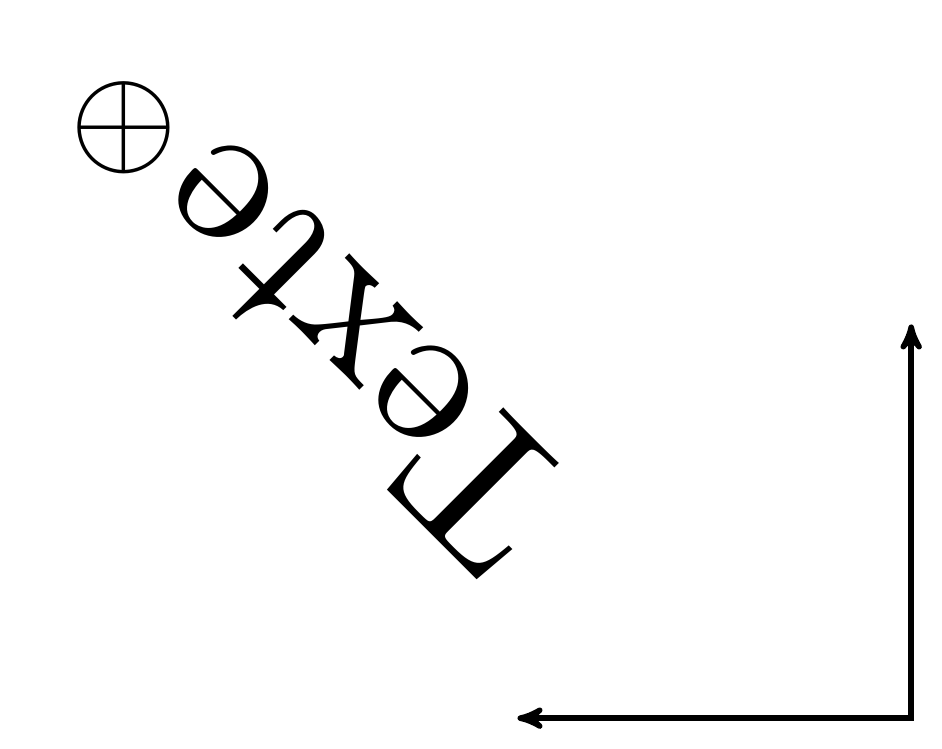
\begin{tikzpicture} [scale=5,rotate=90,transform shape]
  % code de la Figure
  \draw[<->,>=stealth',line width=2pt] (1,0)--(0,0)--(0,1);
  \path (1.5,2) node{$\oplus$}
                node[left,scale=1.5,rotate=45]{Texte};
\end{tikzpicture}}
\end{center}

\end{document}
